\documentclass{article}

\usepackage{graphicx}
\usepackage{tabularx}

\title{\Huge Compte Rendu Hashtable}
\date{19-02-2024}
\author{Wilhem Blondel (21212622) et Alexandre Genin (21131809)}

\begin{document}
    \pagenumbering{gobble}
    \maketitle
    \newpage
    \pagenumbering{arabic}

    \section{Introduction}
    Dans ce TME, l'objectif était de comparer la différence de temps de calcul
    entre une liste chaînée et une table de hachage, en particulier dans les fonctions
    de recherches. La mise en situation ici, consiste à gérer les livres d'une
    bibliothèque dans ces 2 structures.
    \newline \newline
    Une liste chaînée est une structure de données récursive, qui consiste à
    faire pointer une cellule vers son élément suivant. Une liste chaînée est 
    constituée d'une cellule tête, qui permet de reconstruire l'intégralité de ses
    données à partir de ses éléments suivants.
    \newline
    Une table de hachage est un tableau de taille fixée $m$. Chaque indice
    correspond au résultat d'une fonction de hachage paramétrée par une
    clé $k$ spécifique (ici la somme ASCII de l'auteur). Parfois, une fonction de hachage peut renvoyer pour deux clés
    différentes, la même valeur. C'est ce que l'on appelle une collision.
    Notre fonction de hachage ici est $\lfloor m(kA-\lfloor kA \rfloor) \rfloor$ où $A$ 
    le nombre d'or de différence 1. Elle limitera le nombre de collisions dans la table si $m$
    est au moins proportionnelle au nombre de livre qu'elle stocke (noté $n$).
    \newline
    Dans ce TME, les collisions sont gérées par des listes chaînées. C'est à dire que
    chaque case de notre table de hachage pointe vers une liste chaînée, et que,
    lors d'une collision, l'élément en question est ajouté à la liste chaînée.
    \newline
    Notre projet est composé de différents fichiers:

    \begin{itemize}
        \item \texttt{Makefile} Qui permet de compiler le tout efficacement
        \item \texttt{biblioLC.c} et \texttt{biblioH.c} qui contient respectivement
        les fonctions essentielles pour créer une bibliotèque en liste chaînée et
        en table de hachage. On y retrouve notamment les fonctions de création et
        de libération des éléments.
        \item \texttt{entreeSortieLC.c} et \texttt{entreeSortieH.c} qui contiennent
        respectivement les fonctions d'entrées sorties essentielles pour les listes chaînées
        et la table de hachage. En particulier les fonctions de recherches qui nous
        permettront de tirer des conclusions quant à l'efficacité de ces deux structures
        \item \texttt{main.c} et \texttt{mainH.c} qui permettent de tester respectivement
        les fonctions des listes chaînées et des tables de hachage. Une interface a été
        programmée pour rendre la chose plus facile.
        \item \texttt{comparaison.c} qui permet de comparer les temps de recherches entre
        une liste chaînée et une table de hachage et dont les résultats ont été explicités
        en Q.3.1
        \item \texttt{courbes.c} qui permet de générer un fichier de données 
        que l'on peut utiliser avec \texttt{gnuplot} et observer les différences
        de temps de calcul pour la recherche de doublons entre une liste chaînée et
        une table de hachage
        \item \texttt{biblioLC.h}, \texttt{entreeSortieLC.h}, \texttt{biblioH.h} et \texttt{entreeSortieH.h}
        permettant d'utiliser les fonctions des fichiers C associées dans d'autre fichiers
    \end{itemize}
    

    \newpage
    \section{Question 3.1 et 3.2}

    Pour effectuer la comparaison de temps de calcul entre la table de hachage, nous avons créé
    le fichier \texttt{comparaison.c} qui effectue 100 recherches consécutives 
    dans la liste chaînée, puis dans la table hachage de taille donnée. 
    \newline
    Les deux structures ont chargé l'intégralité de la bibliothèque de 100000 livres,
    l'élément recherché "connu" était le même à chaque test et avait une position éloignée
    d'environ 77000 blocs de la tête de liste chaînée.
    \newline
    Les résultats observés sont les suivants:

    \begin{table}[h]
        \centering
            \begin{tabularx}{\textwidth}{ |*{5}{>{\centering\arraybackslash}X|} }
                \hline
                Type de recherche& Liste chaînée & Hastable (500 clés)  & Hashtable (50 clés) & Hashtable \newline (5 clés)\\
                \hline
                Numéro connu & 0.014844 ms & 0.237934 ms & 0.205067 ms &  0.157843 ms\\
                Numéro inconnu & 0.088723 ms & 0.510378 ms & 0.491641 ms & 0.343747 ms\\
                \hline
                Titre connu & 0.020914 ms & 0.299899 ms & 0.284141 ms & 0.227464 ms\\
                Titre inconnu & 0.098122 ms & 0.494885 ms & 0.500609 ms & 0.325849 ms \\
                \hline
                Auteur connu & 0.091525 ms & 0.000130 ms & 0.005319 ms & 0.036859 ms \\
                Auteur inconnu & 0.092567 ms & 0.000166 ms & 0.005531 ms &  0.037656 ms \\
                \hline
            \end{tabularx}
        \caption{Temps de recherche d'une même donnée sur différentes structures}
        \label{tab:hashVSLC}
    \end{table}

    On peut observer ici que la taille de la Hashtable influe en partie sur la vitesse de recherche.
    \newline
    Lorsque l'on recherche selon l'auteur, une table de hachage avec une taille plus importante
    est plus efficace qu'une table ayant une taille plus faible. Ce résultat n'est pas surprenant
    car une table avec une taille plus importante minimise les collisions.
    \newline
    Remarquons néanmoins que peu importe la taille de la table de hachage, le temps de recherche
    est significativement moins important que dans une liste chaînée quand il s'agit de chercher l'auteur.
    \newline
    En revanche observons que le temps de recherche est plus important dans une table de hachage que
    dans une liste chaînée lorsque l'on recherche par numéro ou par titre. Ceci est dû au fait que la
    clé de la table ne dépend pas de ces informations. Ce résultat était effectivemment prévisible.
    \newline
    Lorsque l'on cherche un livre par son numéro, on cherche d'abord dans une certaine case du tableau,
    et on parcourt la liste chaînée associée à cette case. Il faut donc le temps de sauter d'une case
    du tableau à l'autre, et le temps de parcours d'une liste chaînée.
    \newline
    On observe donc de façon logique que plus la table de hachage est petite, plus la recherche à partir
    d'un numéro ou d'un titre est moindre (moins de case à évaluer).
    
    \newpage
    \section{Question 3.3 et 3.4}
    
    Pour effectuer cette comparaison, nous avons préparé un nouveau code: 
    \texttt{courbes.c}
    \newline
    Ce code nous permet d'exécuter la fonction de recherche de doublons sur 
    différentes tailles de bibliothèque, et de comparer le temps d'exécution
    entre une liste chaînée et une table de hachage.
    \newline
    Au début, nous avons décidé d'adapter la taille du tableau de hachage en
    fonction du nombre de livres qu'il contient. (Pour $n$ livres sa taille
    était de $\frac{n}{2}$). 
    \newline
    Mais étant donné le temps de calcul relativement rapide de la Hastable
    par rapport à la liste chaînée, nous avons fixé son nombre de clés à 20,
    pour éviter de n'observer qu'une courbe plate (non représentative des 
    observations attendues)
    \begin{figure}[h]
        \centering
        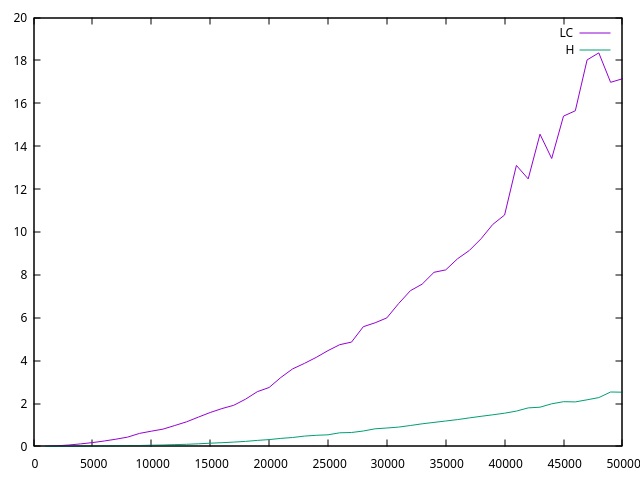
\includegraphics[width=0.55\textwidth]{graph.png}
        \caption{Temps de calcul entre une liste chaînée et hashtable de 20 clés}
        \label{fig:hash20}
    \end{figure}
    \newline
    D'après Q.3.2, le temps de calcul est plus long, permettant de mieux commenter.
    \newline
    Observons que la croissance de la courbe verte (le temps de calcul de la hastable en fonction du nombre d'entrées)
     est significativement moins importante que
    celle de la liste chaînée (en violet). 
    \newline
    Notons $n$ le nombre de livres: La fonction
    de recherche de doublons dans la liste chaînée va itérer autant dans le pire et meilleure des cas:
    Pour le premier élément, on le compare à $n-1$ éléments, puis le second à $n-2$ etc.
    D'où:
    $$ \Theta\left(\sum^{n-1}_{i=0} i\right)  = \Theta\left(\frac{(n-1)n}{2}\right) = \Theta(n^2)$$  
    \newline
    Dans la table de hachage, on a dans le pire cas, $\mathcal O(n^2)$
    (Tous les éléments ont la même valeur au hachage, donc on itère sur une liste chaînée classique).
    \newline
    Dans le cas général,
    En notant $m$, la taille de notre table de hachage, et $p$ le nombre d'éléments dans une 
    case de la table de hachage,
    la complexité cas général est de $\Theta(mp^2)$ où $p << n$ (car on limite les collisions un maximum).
    \newline
    On cherche donc des doublons dans des listes chaînées nettement moins grande.
    Ceci explique donc les différences de croissance observées.

        
\end{document}
